%ekg_7_Realisierung/analoge_Filterschaltung

\subsection{Analoge Filterschaltung}

Dieses Unterkapitel behandelt die Analyse der Anforderungen eines EKG-Signals und wie diese in der analogen Filterschaltung umgesetzt wurden. Wie bereits im Kapitel Einleitung und Motivation erklärt wurde, soll das EKG-Gerät das Signal über einen Kanal messen. Hierfür wird die Differenz zwischen zwei Klebeelektroden, die der Benutzer an seiner Brust befestigt, gebildet. Für die Differenzbildung wird der Instrumentenverstärker AD8422ARMZ von Analog Devices (AD) verwendet. Dieser Rail-to-Rail-Verstärker erreicht im niedrigen Frequenzbereich bis \SI{60}{\hertz} eine Gleichtaktunterdrückung von etwa \SI{120}{\decibel}, was Störsignale die durch externe elektromagnetische Felder in die Messleitungen eingekoppelt werden unterdrückt. Seine Verstärkung wird mittels eines \SI{33}{\ohm}-Widerstandes auf den Faktor 420 eingestellt, was etwa in \SI{52}{\decibel} entspricht. Diese Vorverstärkung sorgt dafür, dass das Signal auf dem Weg durch die Filterschaltung robuster gegen Störungen ist. Da das Endprodukt über einen Akku betrieben wird, ist der Instrumentenverstärker fähig mit einer einseitigen Versorgungsspannung zu arbeiten und benötigt einen geringen Versorgungsstrom von etwa \SI{330}{\micro\ampere}. Die vor den Eingängen des Differenzverstärkers liegende Eingangstufe ist hochohmig um die Signalquelle, also den Körper nicht zu belasten, da ansonsten die Signalstärke einbrechen würde. Die beiden Kanäle sind symmetrisch aufgebaut und bestehen jeweils aus einer bidirektionalen TVS-Diode, einem passiven Hochpass und einem passiven Tiefpass. Die Diode dient dazu Überspannung bei einer elektrostatischen Entladung (ESD) abzuleiten und so die dahinter liegende Schaltung zu schützen. Der Hochpass mit einer Grenzfrequenz von \SI{0,48}{\hertz} trennt den Gleichanteil des Signal ab, welcher durch den Übergang von Ionen- zu Elektronenleitung an der Kontaktfläche der Elektroden entsteht. Zudem koppelt er das Kleinsignal des EKGs in das Gleichspannungspotential von \SI{1,5}{\volt} der Filterschaltung ein. Die Schaltung wird auf dieses Potenzial angehoben, um auch die negativen Signalanteile (Q- und S-Zacke des EKGs) übertragen zu können, was aufgrund der einseitigen Versorgungsspannung sonst nicht möglich wäre. Der Tiefpass mit einer Grenzfrequenz von \SI{159}{\hertz} dient dazu hochfrequente (>\SI{100}{\kilo\hertz}) Störungen bereits vor dem Instrumentenverstärker zu unterdrücken. Um einen Eindruck vom Frequenzspektrum eines EKG-Signals zu erhalten, wurde mit Matlab ein künstliches EKG-Signal (siehe Abbildung 1) aus Kosinusfunktionen und linearen Funktionen erstellt. Aus der im Anschluss durchgeführten Fast-Fourier-Transformation (FFT) (siehe Abbildung 2), lässt sich erkennen, dass die stärksten Frequenzanteile bis etwa \SI{40}{\hertz} gehen. Da jedoch gerade die hochfrequenten Anteile des Signals für die Ausformung der charakteristischen QRS-Zacken verantwortlich sind, wurde die obere Grenzfrequenz der Filterschaltung auf \SI{159}{\hertz} gesetzt. 

\begin{figure} [!h]
	%\centering
	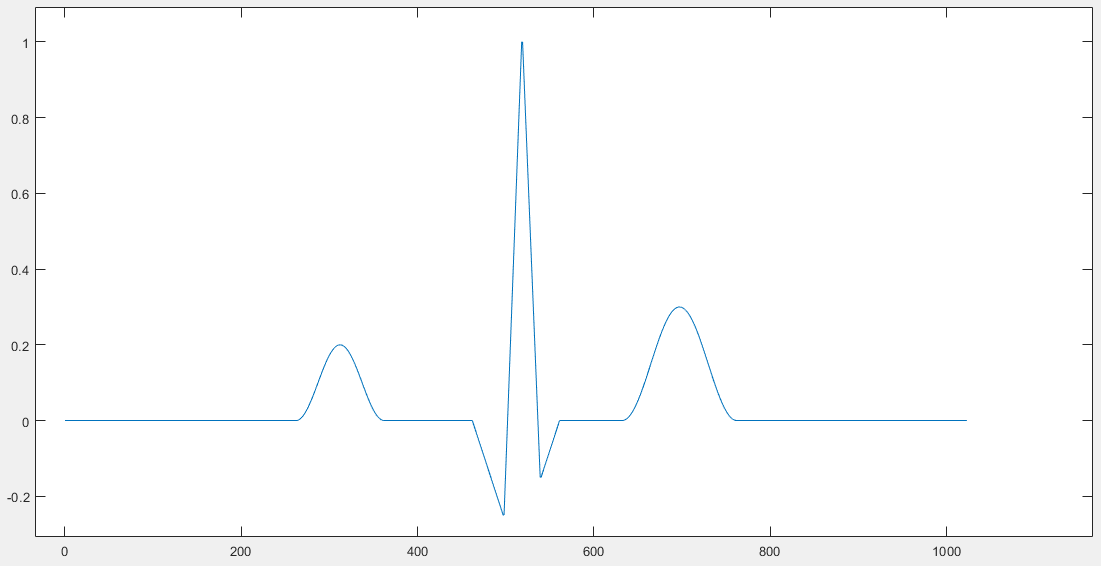
\includegraphics[width=\textwidth] {EKG_Signal.png}
	\caption{mit Matlab erstelltes künstliches EKG-Signal}
	\label{fig1} 
\end{figure}

\begin{figure} [!h]
	%\centering
	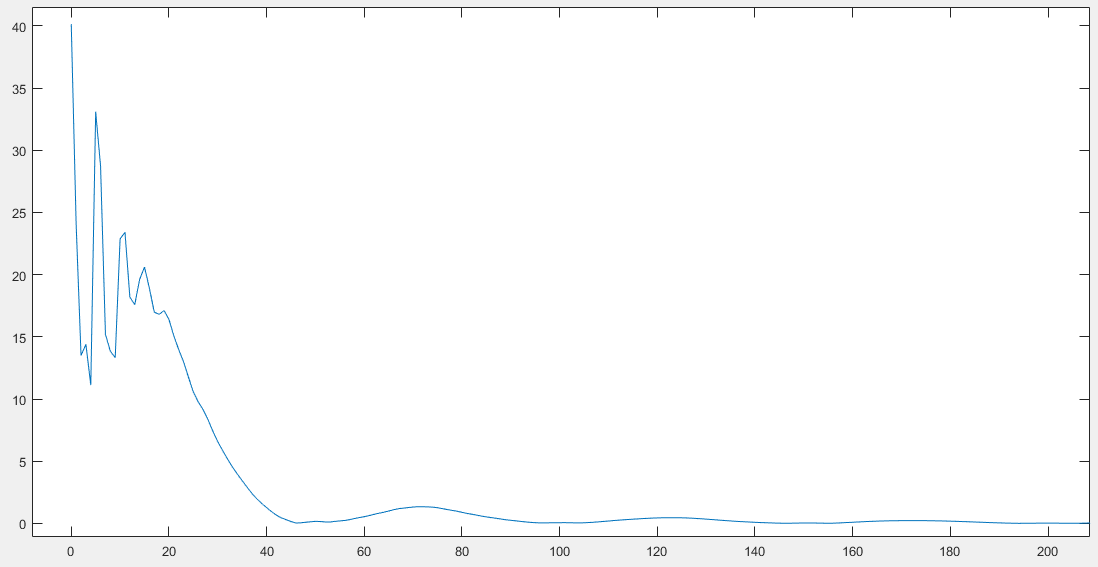
\includegraphics[width=\textwidth] {EKG_diskretes_Frequenzspektrum_Ausschnitt.png}
	\caption{Frequenzspektrum des künstlichen EKG-Signals}
	\label{fig2} 
\end{figure}

Da der Körper eines Menschen aus leitendem Material besteht, können elektromagnetische Wechselfelder, wie die von Stromleitungen in Hauswänden, eine Spannung in ihm induzieren. Diese Wechselspannung, mit einer Amplitude von bis zu \SI{100}{\milli\volt} und einer Frequenz von \SI{50}{\hertz} überlagert das EKG-Signal des Herzens. Um dieses Netzrauschen zu unterdrücken, wird ein Doppel-T-Filter verwendet. Bei idealen Bauteilen erreicht diese aktive Bandsperre eine Güte von annähernd 0,5 und eine Dämpfung von \SI{76}{\decibel}. Da jedoch die verwendeten SMD-Widerstände und Kondensatoren nur mit gewissen Toleranzen erhältlich sind, fällt die effektive Dämpfung auf \SI{20}{\decibel} bis \SI{30}{\decibel}. Dies wäre für die Anwendung nicht ausreichend, daher werden in der Schaltung zwei dieser Bandsperren in Reihe geschaltet. Die im Schaltplan vorgesehenen Parallelschaltungen der Widerstände dienen dazu die Widerstandswerte flexibel einzustellen, um auch noch im Nachhinein auf die Toleranzen der Kondensatoren reagieren zu können. Bei den benötigten Operationsverstärkern wurde ein vier in eins Bauteil von AD gewählt. Zwei der Operationsverstärker werden für die \SI{50}{\hertz}-Filter verwendet, die anderen zwei dienen der Tiefpassfilterung und Nachverstärkung. Der AD8544ARZ ist ein einseitig versorgbarer Rail-to-Rail-Verstärker mit einem geringen Versorgungsstrom von \SI{45}{\micro\ampere}. Da das zu filternde Signal im niederfrequenten Bereich liegt, ist er mit seinem Verstärkungs-Bandbreite-Produkt von \SI{1}{\mega\hertz} mehr als ausreichend. Mit dem Analog-Digital-Umsetzer (ADC) wird eine Abtastfrequenz von \SI{1}{\kilo\hertz} angestrebt. Das Signal wird daher durch Tiefpässe begrenzt. Die Tiefpassfilterung setzt sich aus vier passiven Tiefpässen erster Ordnung und einem aktiven Tiefpass zweiter Ordnung zusammen. Die passiven Filter sind zwischen die aktiven Stufen der Schaltung eingebettet.

\begin{figure} [!h]
	%\centering
	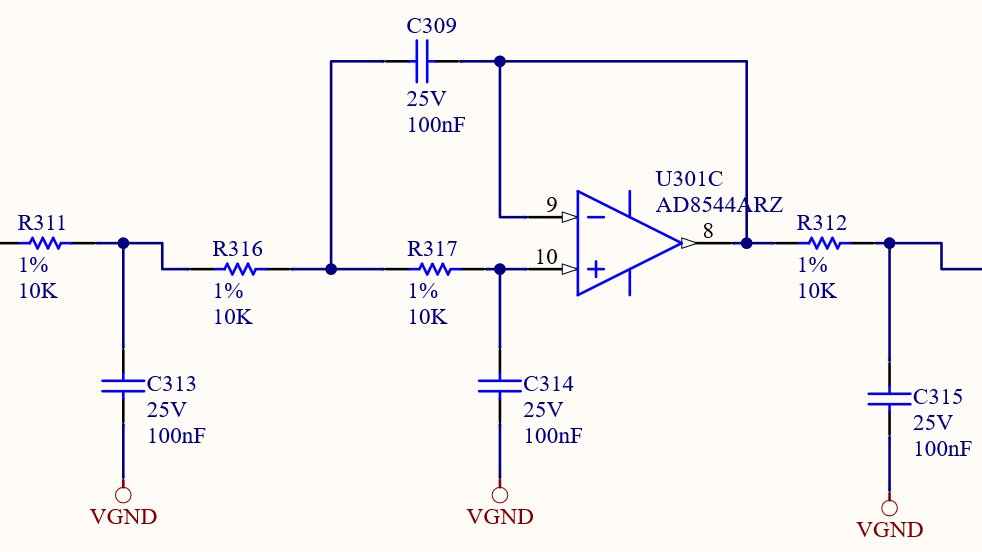
\includegraphics[width=\textwidth] {EKG_aktiver_Tiefpassfilter.png}
	\caption{aktiver Tiefpass eingeschlossen von zwei passiven Tiefpässen}
	\label{fig3} 
\end{figure}

In Abbildung 3 ist der verwendete aktive Tiefpass, realisiert durch eine Sallen-Key-Schaltung abgebildet. Davor und dahinter befinden sich einfache passive Tiefpässe. Die zwei verbleibenden passiven Tiefpassfilter befinden sich in der Eingangsstufe (je einer pro Kanal) und zwischen den beiden \SI{50}{\hertz}-Filtern. Insgesamt ergibt sich damit eine Tiefpassfilterung sechster Ordnung, also eine Dämpfung von \SI{120}{\decibel} pro Dekade, über die gesamte Schaltung. Die Signalamplitude der Quelle beträgt nur etwa \SI{1}{\milli\volt}. Der ADC arbeitet in einem Bereich von \SI{0}{\volt} bis \SI{3}{\volt}, um diesen Bereich bestmöglich auszunutzen muss das Signal auf eine Amplitude von etwa \SI{2}{\volt} verstärkt werden. \SI{1}{\volt} des ADC-Intervalls bleibt als Reserve ungenutzt, um bei Schwankungen des Signals nicht sofort die Begrenzung der Spannungsversorgung zu überschreiten, außerdem kann die Amplitude des Eingangssignals je nach Mensch auch leicht variieren. Insgesamt wird also eine Verstärkung etwa um den Faktor 2000 benötigt, was \SI{66}{\decibel} entspricht. Wie bereits erwähnt, wird durch den Differenzverstärker am Eingang eine Verstärkung von etwa \SI{52}{\decibel} realisiert. Die Filterstufen in der Schaltung bewirken eine Dämpfung des gesamten Signals um etwa \SI{6}{\decibel}, somit muss die Nachverstärkung \SI{20}{\decibel} betragen um die geforderte Gesamtverstärkung von \SI{66}{\decibel} zu erreichen. Dies bewirkt ein nicht-invertierender Spannungsverstärker, mit einem Verstärkungsfaktor von 10, der sein Ausgangssignal direkt auf den Pin des ADCs gibt.

\begin{figure} [!h]
	%\centering
	\includegraphics[width=\textwidth] {EKG_Gesamtübertragungsfunktion.png}
	\caption{Gesamtübertragungsfunktion der Filterschaltung}
	\label{fig4} 
\end{figure}

In Abbildung 4 ist die simulierte Gesamtübertragungsfunktion der Filterschaltung in einer doppelt-logarithmischen Darstellung abgebildet. Für Frequenzen kleiner als \SI{0,5}{\hertz} wird das Signal mit \SI{20}{\decibel} pro Dekade gedämpft, ab \SI{160}{\hertz} wird es durch die Tiefpässe mit \SI{120}{\decibel} pro Dekade unterdrückt. Außerdem gibt es bei \SI{50}{\hertz} eine Dämpfung von \SI{40}{\decibel} von den Bandsperren. Hierbei ist zu beachten, dass die Simulation mit idealen Bauteilen durchgeführt wurde. In der realen Schaltung fällt die Dämpfung wesentlich geringen aus, sodass die Übertragungsfunktion in diesem Bereich bei zirka \SI{0}{\decibel} liegt. Für den übrigen Frequenzbereich wird eine Verstärkung um \SI{67}{\decibel} erreicht. Der Gesamtschaltplan der Filterung befindet sich in Anhang \textit{(Anhang wurde noch nicht erstellt)}. 

\begin{figure} [!h]
	%\centering
	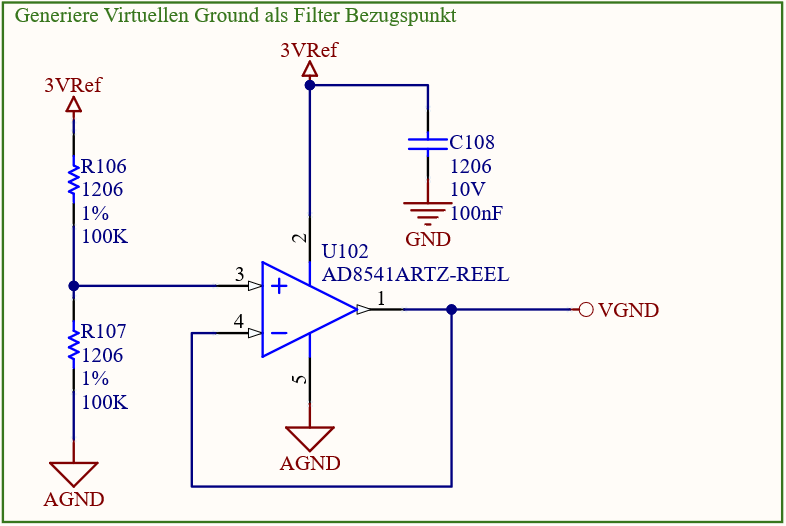
\includegraphics[width=\textwidth] {EKG_virtueller_Ground.png}
	\caption{Generierung des 1,5 V Bezugspotentials für die Filterschaltung}
	\label{fig5} 
\end{figure}

Um die Schaltung auf ein Gleichspannungspotenzial von \SI{1,5}{\volt} anzuheben wurde ein hochohmiger Spannungsteiler mit einem Operationsverstärker als Spannungsfolger verwendet. Bei dem Operationsverstärker handelt es sich um den AD8541ARTZ-REEL. Es ist der gleiche Verstärker der auch für die Filter zum Einsatz kommt, nur in einem Single-Gehäuse.




